\documentclass[conference]{IEEEtran}
\IEEEoverridecommandlockouts

\usepackage{cite}

\usepackage{graphicx}

\usepackage[T1]{fontenc}
\usepackage[utf8]{inputenc}
\bibliographystyle{ieeetr}

\author{\IEEEauthorblockN{Michał Klemens, 266883}
\IEEEauthorblockA{Politechnika Wrocławska \\
Informatyka Stosowana\\
5 Czerwiec, 2023}
}


\begin{document}

\title{Klasyfikacja obiektów gwiezdnych na podstawie charakterystyki spektralnej}




\maketitle

\section{Wstęp}
Kategoryzacja gwiazd, galaktyk i kwazarów na podstawie ich właściwości spektralnych jest kluczowym pojęciem w astronomii. Dzieląc gwiazdy na różne kategorie w oparciu o czynniki takie jak ich temperatura, jasność i skład chemiczny, możemy uzyskać wgląd w ich właściwości fizyczne i etapy ewolucji. Wczesne próby katalogowania gwiazd i ich położenia na niebie doprowadziły do odkrycia, że są one częścią naszej własnej galaktyki, a gdy teleskopy stały się bardziej zaawansowane, ustalono, że istnieją inne galaktyki, takie jak Andromeda, co zapoczątkowało dalsze badania.
Aby lepiej zrozumieć raport należy zapoznać się z opisem każdej z klas:
\begin{itemize}
    \item \textbf{Gwiazda}, jej życie rozpoczyna się od grawitacyjnego zapadnięcia się mgławicy gazowej składającej się głównie z wodoru, helu i śladowych ilości cięższych pierwiastków. Jej całkowita masa jest głównym czynnikiem determinującym jej ewolucję i ostateczny los. Gwiazda świeci przez większość swojego aktywnego życia dzięki termojądrowej fuzji wodoru w hel w swoim jądrze. Proces ten uwalnia energię, która przemierza wnętrze gwiazdy i promieniuje w przestrzeń kosmiczną. Pod koniec życia gwiazdy jej jądro staje się gwiezdną pozostałością: białym karłem, gwiazdą neutronową lub - jeśli jest wystarczająco masywna - czarną dziurą.
    \begin{figure}[ht]
        \centering
        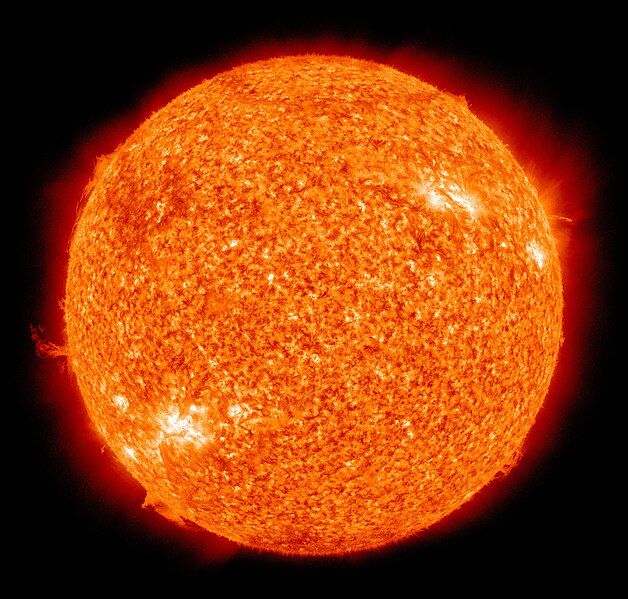
\includegraphics[width = 5cm]{figures/star.jpg}
        \caption{Słońce, najbliższa Ziemi gwiazda.\cite{star}}
    \end{figure}
    \item \textbf{Galaktyka} to układ gwiazd, pozostałości gwiezdnych, gazu międzygwiezdnego, pyłu i ciemnej materii powiązanych ze sobą grawitacyjnie. Większość masy w typowej galaktyce ma postać ciemnej materii, a tylko kilka procent tej masy jest widoczne w postaci gwiazd i mgławic. Ponadto w centrach galaktyk często spotykane są supermasywne czarne dziury.
    \begin{figure}[ht]
        \centering
        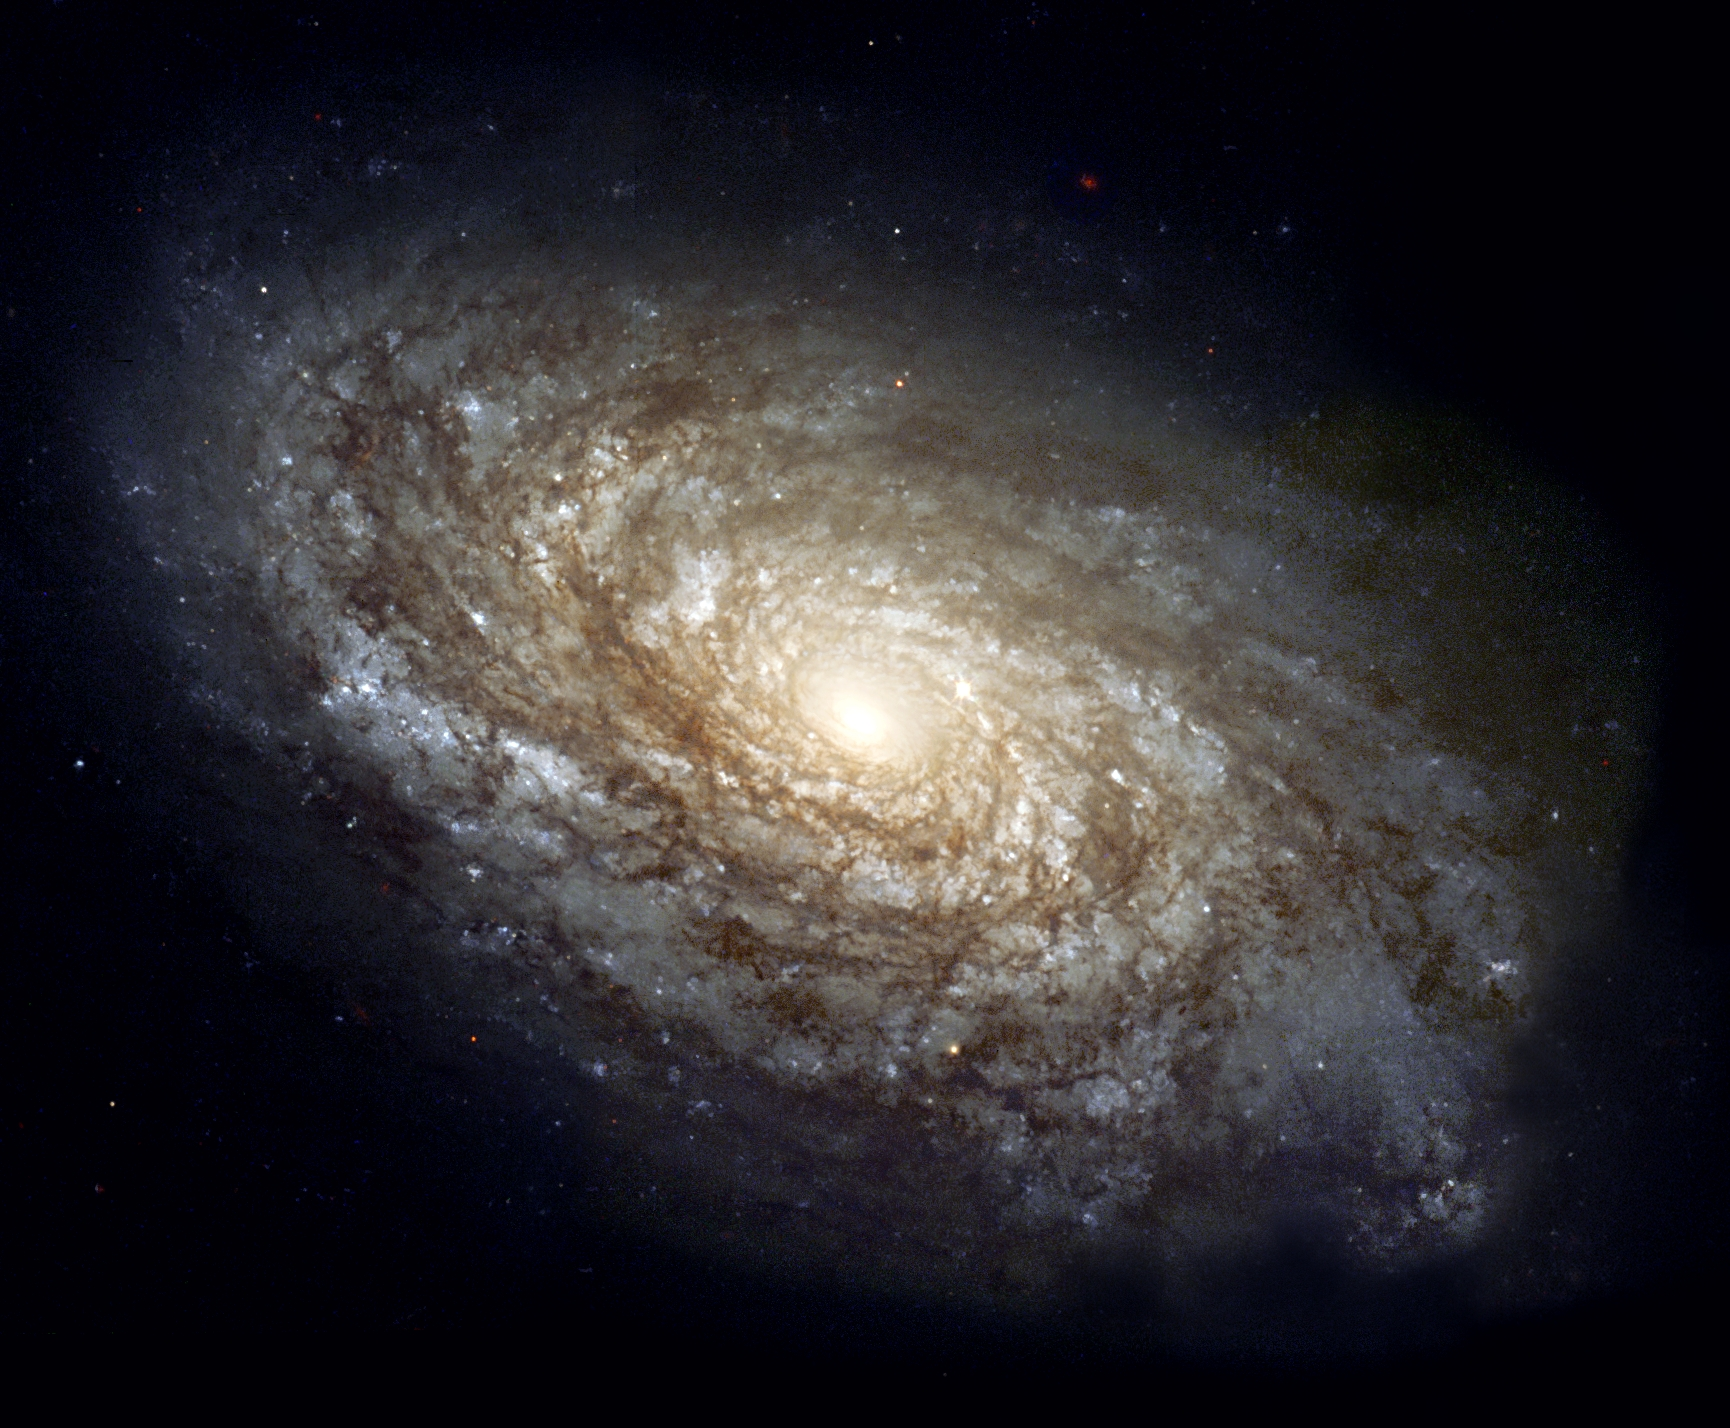
\includegraphics[width = 5cm]{figures/galaxy.jpg}
        \caption{NGC 4414, typowa galaktyka spiralna w konstelacji Coma Berenices\cite{galaxy}}
    \end{figure}
    \item \textbf{Kwazar} to niezwykle jasne aktywne jądro galaktyczne. Emisja światła z kwazaru jest powodowana przez supermasywną czarną dziurę o masie od milionów do dziesiątek miliardów mas Słońca, otoczoną gazowym dyskiem akrecyjnym. Gaz w dysku opadający w kierunku czarnej dziury nagrzewa się z powodu tarcia i uwalnia energię w postaci promieniowania elektromagnetycznego. Energia promieniowania kwazarów jest ogromna; najpotężniejsze kwazary mają jasność tysiące razy większą niż galaktyki takie jak Droga Mleczna.
    \begin{figure}[ht]
        \centering
        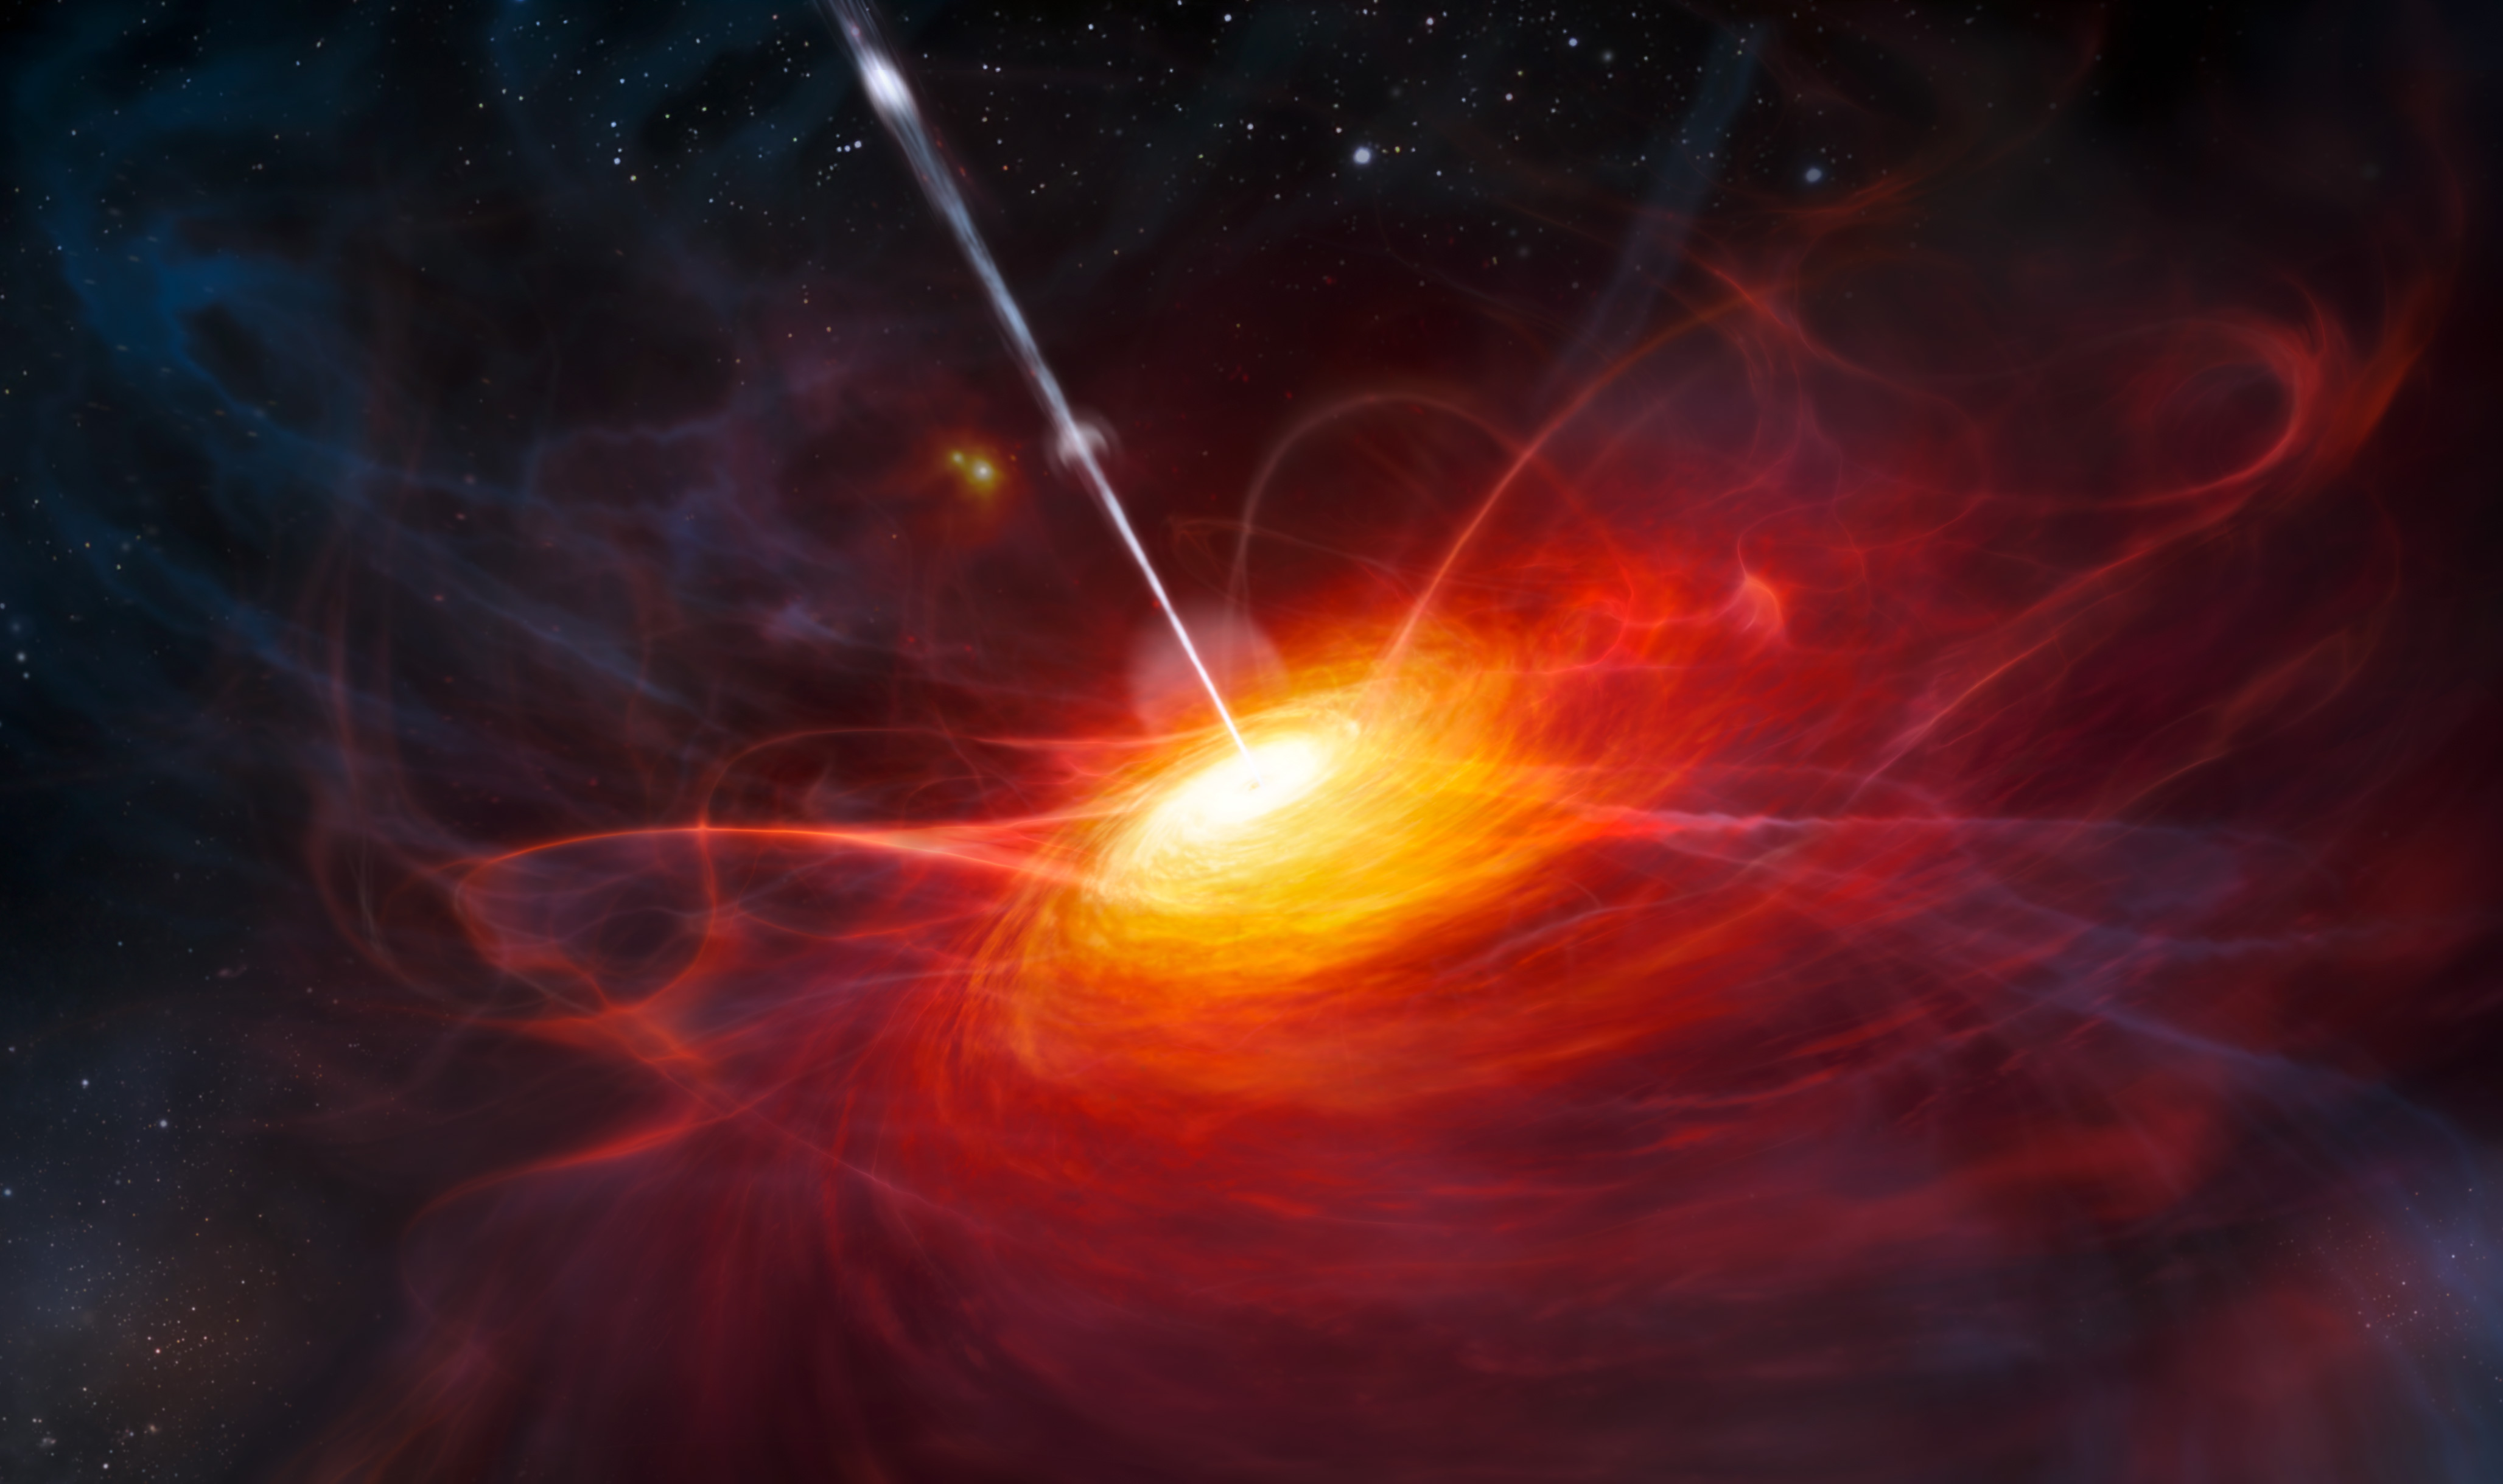
\includegraphics[width = 5cm]{figures/quazar.jpg}
        \caption{Impresja artystyczna pokazująca, jak mógł wyglądać ULAS J1120+0641, bardzo odległy kwazar zasilany przez czarną dziurę o masie dwa miliardy razy większej niż masa Słońca.\cite{quasar}}
    \end{figure}
\end{itemize}
\section{Dane i ich przygotowanie}
Dane składają się ze 100 000 obserwacji przestrzeni kosmicznej wykonanych przez SDSS (Sloan Digital Sky Survey). Każda obserwacja jest opisana przez 17 kolumn cech i 1 kolumnę klasy, która identyfikuje ją jako gwiazdę, galaktykę lub kwazar. Lista cech:
\begin{itemize}

    \item \textbf{obj\_ID} - identyfikator obiektu to unikalna wartość, która identyfikuje obiekt w katalogu obrazów używanym przez archiwum danych Sloan Digital Sky Survey (SDSS),
    \item \textbf{alpha} - rektascensja w epoce J2000, jedna ze współrzędnych astronomicznych, określających położenie ciała niebieskiego na sferze niebieskiej,
    \item \textbf{delta} - deklinacja w epoce J2000, jedna ze współrzędnych astronomicznych, określających położenie ciała niebieskiego na sferze niebieskiej,
    \item \textbf{u, g, r, i, z} - to filtry fotometryczne używane w systemie SDSS do pomiaru ilości światła z obiektów w różnych zakresach długości fal. Każdy filtr odpowiada innemu kolorowi światła, przy czym \textbf{u} to zakres ultrafioletu, \textbf{g} - zieleni, \textbf{r} - czerwieni, \textbf{i} - bliskiej podczerwieni, a \textbf{z} - podczerwieni,
    \item \textbf{run\_ID} - numer przebiegu służy do identyfikacji konkretnego skanu nieba wykonanego przez SDSS. Każdy skan obejmuje określony obszar nieba i ma przypisany unikalny numer przebiegu,
    \item \textbf{rerun\_ID} - numer ponownego uruchomienia służy do określenia sposobu przetwarzania obrazu
    \item \textbf{cam\_col} - kolumna kamery służy do identyfikacji linii skanowania w przebiegu. Każdy skan jest podzielony na wiele kolumn kamer, aby objąć większy obszar nieba,
    \item \textbf{field\_ID} - numer pola służy do identyfikacji każdego pola w skanowaniu, które jest mniejszym obszarem w kolumnie kamery,
    \item \textbf{spec\_obj\_ID} - unikalny identyfikator używany dla obiektów spektroskopii optycznej. Oznacza to, że dwie różne obserwacje z tym samym identyfikatorem \textbf{spec\_obj\_ID} muszą dzielić klasę wyjściową, którą jest galaktyka, gwiazda lub kwazar,
    \item \textbf{class} - klasa obiektu, przypisana mu na podstawie jego charakterystyki spektralnej. Może być to galaktyka,\\ gwiazda lub kwazar,
    \item \textbf{redshift} - wartość przesunięcia ku czerwieni opiera się na wzroście długości fali światła emitowanego przez obiekt z powodu jego ruchu od lub w kierunku obserwatora,
    \item \textbf{plate} - identyfikator płytki identyfikuje każdą płytkę używaną w badaniu spektroskopowym SDSS. Każda płytka zawiera wiele włókien, które zbierają światło z różnych obiektów,
    \item \textbf{MJD} - zmodyfikowana data juliańska, używana do wskazania, kiedy dany fragment danych SDSS został pobrany.
    \item \textbf{fiber\_ID} - identyfikator włókna, który identyfikuje włókno, które skierowało światło na płaszczyznę ogniskową w każdej obserwacji.
\end{itemize}

Raport skupia się na analizie charakterystyki spektralnej. Zatem można odrzucić wszystkie cechy pełniące rolę identyfikatora. To znaczy: \textbf{run\_ID}, \textbf{rerun\_ID}, \textbf{field\_ID}, \textbf{spec\_obj\_ID}, \textbf{fiber\_ID}, a także \textbf{plate} i \textbf{cam\_col}. Dodatkowo data wykonania obserwacji \textbf{MJD} oraz cechy: deklinacja (\textbf{delta}) i rektascensja (\textbf{alpha}), które stanowią o położeniu obiektu na mapie nieba, również można odrzucić. \\
Pozostałe cechy stanowią o charakterystyce spektralnej obiektu (\textbf{u}, \textbf{g}, \textbf{r}, \textbf{i}, \textbf{z} oraz \textbf{redshift}) i to własnie one będą wykorzystywane w rozwiązaniu problemu klasyfikacji.
\section{Analiza eksploracyjna}
Analizując dane można zauważyć znaczącą dysproporcję w liczebności poszczególnych klas. Zbiór zawiera 59445 galaktyk (ang. galaxy), 18961 kwazarów (ang. quasar) oraz 21594 gwiazd (ang. star), co ilustruje poniższy wykres. 
\begin{figure}[ht]
        \centering
        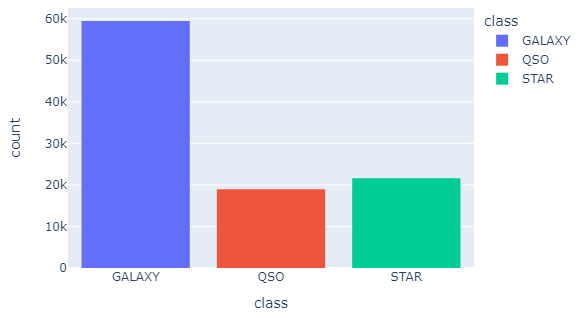
\includegraphics[width = 8cm]{figures/class_count.png}
        \caption{Wykres liczebności każdej klasy obiektu w zbiorze danych}
\end{figure} \\

Jako ciekawostkę można przedstawić również mapę nieba, obrazującą położenie każdego badanego obiektu na niebie. 

\begin{figure}[ht]
        \centering
        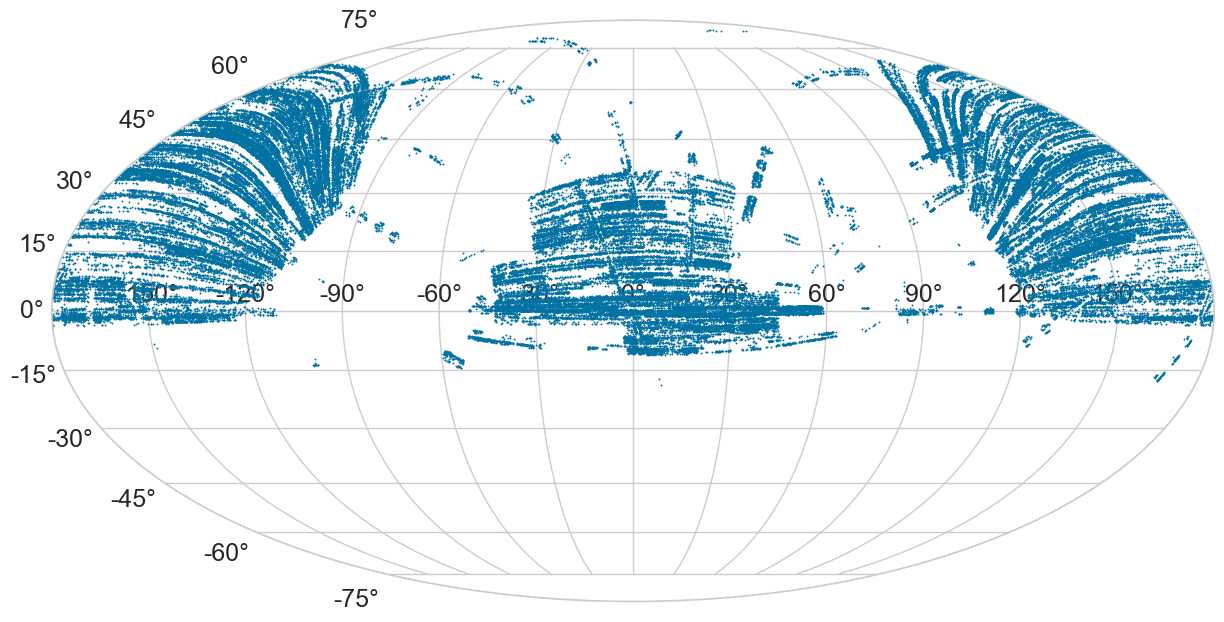
\includegraphics[width = 8cm]{figures/celestial_map.png}
        \caption{Mapa nieba wraz z zaznaczonymi na niej wszystkimi obiektami w zbiorze danych.}
\end{figure}
Korelacje cech z klasą obiektu przedstawione są w tabeli (Table I). Jak widać największą korelację z klasą obiektu mają cechy \textbf{redshift} (0,536) oraz \textbf{i} (0,284). Można zauważyć, że cechy będące identyfikatorami w większości mają znikomą korelację z klasą obiektu. Co również przemawia za odrzuceniem owych cech ze zbioru. Należy dodać, że cecha \textbf{rerun\_ID} w całym zbiorze przyjmuje tylko jedną wartość, dlatego nie jest ujęta w tabeli. 


\begin{table}[ht]
    \centering
    \begin{tabular}{|l|r|}
        \hline
        Cecha & Korelacja \\
        \hline
        field\_ID & -0,038 \\
        \hline
        u & -0,017 \\
        \hline
        g & 0,005 \\
        \hline
        run\_ID & 0,000 \\
        \hline
        obj\_ID & 0,000 \\
        \hline
        alpha & 0,004 \\
        \hline
        cam\_col & 0,014 \\
        \hline
        z & 0,017 \\
        \hline
        fiber\_ID & 0,032 \\
        \hline
        delta & 0,056 \\
        \hline
        r & 0,150 \\
        \hline
        MJD & 0,207 \\
        \hline
        spec\_obj\_ID & 0,215 \\
        \hline
        plate & 0,215 \\
        \hline
        i & 0,284 \\
        \hline
        redshift & 0,536 \\
        \hline
        
    \end{tabular}
    \caption{Korelacja cech z klasą obiektu}
\end{table} 

Wykrywanie wartości odstających zostało przeprowadzone przy użyciu metody rozstępu międzykwartylowego (ang. interquantile range, IQR). Metoda ta polega na obliczeniu pierwszego (\textit{Q1}) oraz trzeciego (\textit{Q3}) kwartyla, a także wspomnianego wcześniej rozstępu, którego wzór wygląda następująco: $IQR=Q3-Q1$. Wartości odstające są definiowane jako obserwacje, które spadają poniżej $Q1 - 1,5 IQR$ lub powyżej $Q3 + 1,5 IQR$. \\ 
Metodę zastosowano dla każdej cechy stanowiącej o charakterystyce spektralnej danej obserwacji. Z jej pomocą odrzucono 8992 obserwacji. 

Poniżej przedstawiono również histogramy oraz wykresy skrzypcowe dla dwóch najbardziej skorelowanych z klasą obiektu cech. 
\begin{figure}[ht]
        \centering
        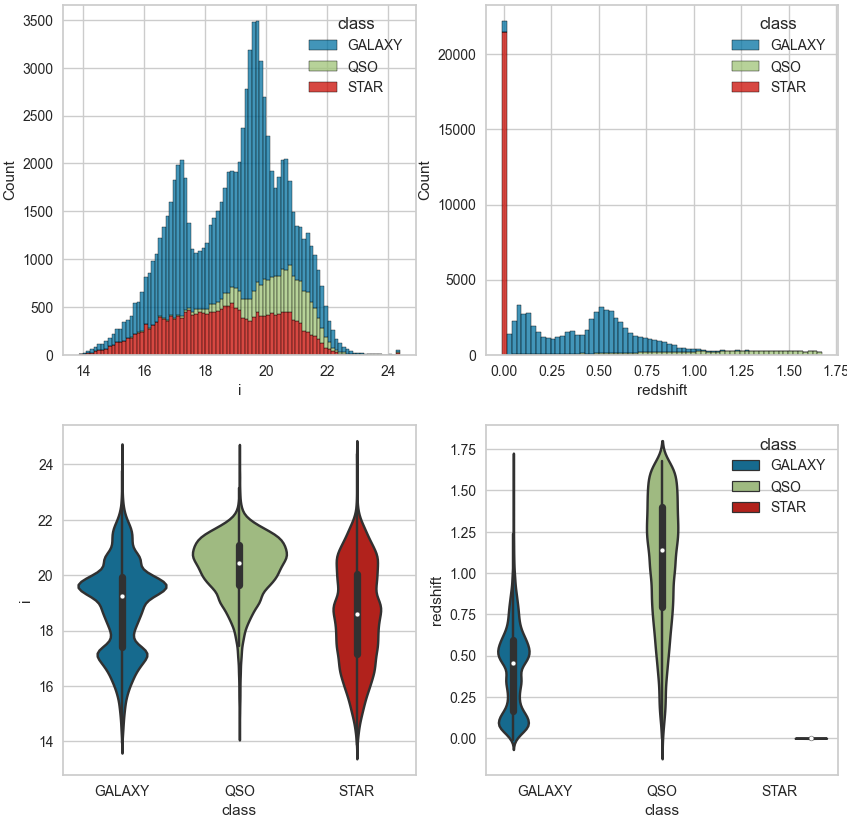
\includegraphics[width = 8cm]{figures/plots.png}
        \caption{Wykresy słupkowe oraz skrzypcowe dla cech: \textbf{i} - lewa kolumna, \textbf{redshift} - prawa kolumna.}
\end{figure} \\
Można zauważyć, że gwiazdy bardzo mocno wyróżniają się na podstawie samej cechy \textbf{redshift}. Ponadto znacząca większość kwazarów ma wyższe wartości tej cechy w porównaniu z resztą klas. Dla cechy \textbf{i} rozkład jej wartości w klasie kwazarów najbardziej się wyróżnia z pozostałych.

Do zbalansowania liczebności każdej z klas przyjęto podejście nadpróbkowania (ang. oversampling). Zapewniło to równą liczbę obserwacji każdej z klas, jednocześnie nie powodując utraty informacji jak w przypadku metody polegającej na usuwaniu danych z klasy większościowej (ang. undersampling).

Skalowanie cech ma kluczowe znaczenie dla niektórych algorytmów uczenia maszynowego, które uwzględniają odległości między obserwacjami. W przypadku SVM, jeśli cechy wejściowe używają różnych skali, to niektóre z nich mogą mieć większy zakres wartości niż inne. Może to sprawić, że SVM położy większy nacisk na cechy o większych skalach, a więc nierównomiernie uwzględnieni poszczególne z nich w procesie uczenia.
Poniżej przedstawiono wykresy pudełkowe (ang. box plot) dla każdej z przeskalowanych cech.
\begin{figure}[ht]
        \centering
        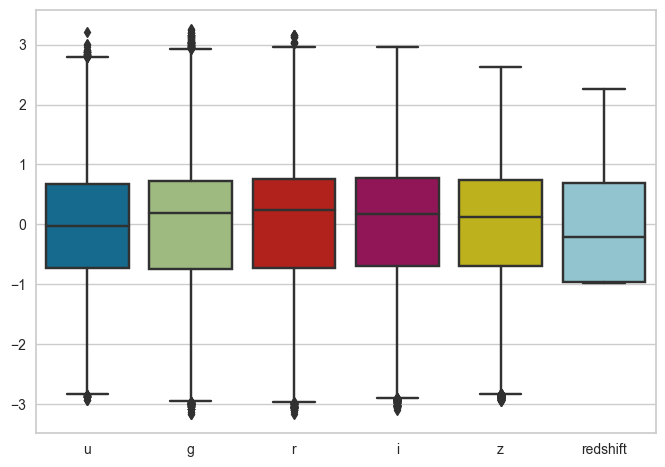
\includegraphics[width = 8cm]{figures/scaled_data.png}
        \caption{Wykresy pudełkowe (ang. box plot) przeskalowanych cech.}
\end{figure} 

Ostatecznie zbiór danych został podzielony na części treningową (około 140 tys. próbek) oraz testową (około 36 tys. próbek).
\section{Klasyfikacja SVM}
Klasyfikacja SVM (Support Vector Machine) to jedna z popularnych metod używanych w dziedzinie uczenia maszynowego do rozwiązywania problemów klasyfikacji. Polega na wyznaczeniu hiperpłaszczyzny - czyli granicy rozdzielającej zbiór na różne klasy - poprzez maksymalizacje odległości (marginesu) hiperpłaszczyzny od próbek najbliższych hiperpłaszczyźnie (wektorów nośnych)
Do rozwiązania problemu zastosowano jądro RBF (Radial Basis Function), które umożliwia skuteczną klasyfikację nawet w przypadku złożonych danych. Separacja każdej z klas odbyła się na zasadzie jeden kontra jeden (ang. one vs one). Z uwagi na ograniczenia związane z mocą obliczeniową, zastosowano domyślne parametry dla SVM.

Poniżej znajduje się tablica pomyłek (ang. confusion matrix) oraz tabela z metrykami dla opisanego wcześniej modelu.
\begin{figure}[ht]
        \centering
        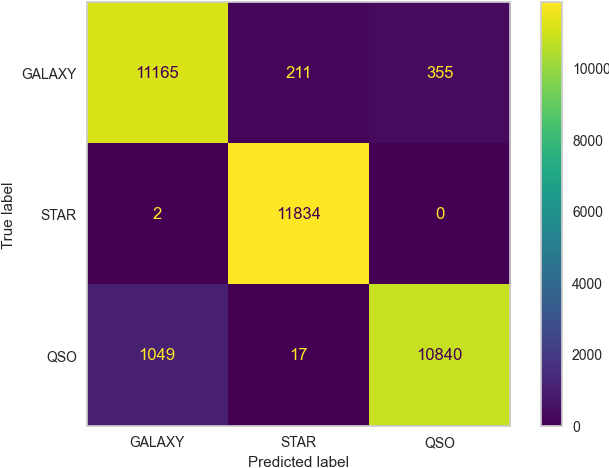
\includegraphics[width = 7.8cm]{figures/svm_conf_mat.png}
        \caption{Tablica pomyłek dla klasyfikacji z użyciem SVM.}
\end{figure} 
\begin{table}[ht]
    \centering
    \begin{tabular}{|l|c|c|c|c|}
        \hline
        Klasa & recall & precision &  F1 & Liczebność\\
        \hline
        Galaktyka & 0.92 & 0.95 & 0.94 & 11731 \\
        \hline
        Gwiazda & 0.98 & 1.00 & 0.99 & 11836 \\
        \hline
        Kwazar & 0.97 & 0.92 & 0.94 & 11906 \\
        \hline
        Średnia aryt. & 0.96 & 0.96 & 0.96 & 35473 \\
        \hline
    \end{tabular}
    \caption{Metryki dla modelu SVM}
\end{table} 

Bazując na tablicy pomyłek jesteśmy w stanie stwierdzić, iż najgorzej model radził sobie z klasyfikacją kwazarów. Ponad tysiąc z nich zostało zaklasyfikowanych jako galaktyki. Natomiast najlepiej wyszła mu klasyfikacja gwiazd - pomylił jedynie dwie gwiazdy klasyfikując je jako galaktyki. 
To samo możemy odczytać z tabeli metryk (Table II). Ogólna celność (ang. accuracy) czyli stosunek dobrze dokonanych klasyfikacji do ilości wszystkich dokonanych klasyfikacji wynosi 0.96. Co jest bardzo dobrym wynikiem. 
\section{Klasyfikacja RF}
 
Las losowy (Random Forest) to metoda oparta na koncepcji łączenia danych wyjściowych wielu drzew decyzyjnych w celu uzyskania pojedynczego wyniku. Ideą lasu losowego jest tworzenie wielu drzew decyzyjnych na podstawie losowego podzbioru danych oraz losowego wyboru cech dla każdego drzewa. Następnie, las losowy łączy wyniki z tych drzew, wybierając klasę, która jest najczęściej wskazywana przez poszczególne drzewa. Dzięki zastosowaniu wielu drzew, las losowy ma zdolność do radzenia sobie z nieliniowymi zależnościami w danych, a także do redukcji efektu przeuczenia (overfitting) dzięki niskiej korelacji między modelami (drzewami), działającymi w grupie.
\begin{figure}[ht]
        \centering
        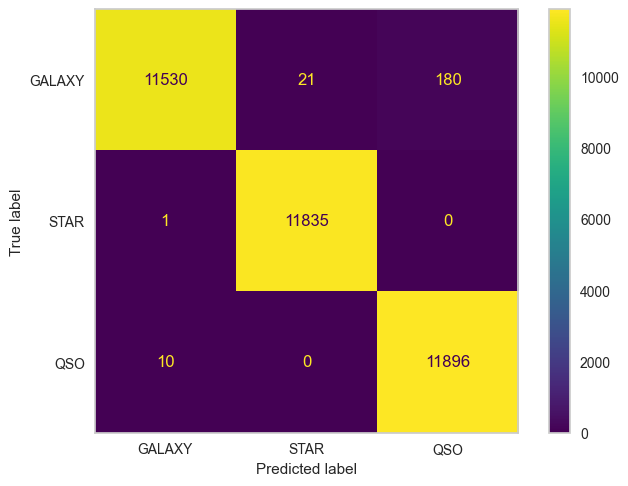
\includegraphics[width = 7.8cm]{figures/rf_conf_mat.png}
        \caption{Tablica pomyłek dla klasyfikacji z użyciem RF.}
        \label{fig:my_label}
\end{figure}
Wyniki działania algorytmu obrazuje tablica pomyłek (Fig. 9) (ang. confusion matrix) oraz tabela z metrykami (Table III).

\begin{table}[ht]
    \centering
    \begin{tabular}{|l|c|c|c|c|}
        \hline
        Klasa & recall & precision &  F1 & Liczebność\\
        \hline
        Galaktyka &  1.00 & 0.98 & 0.99 & 11731 \\
        \hline
        Gwiazda &  1.00 & 1.00 &  1.00 & 11836 \\
        \hline
        Kwazar & 0.98 &  1.00 & 0.99 & 11906 \\
        \hline
        Średnia aryt. & 0.99 & 0.99 & 0.99 & 35473 \\
        \hline
    \end{tabular}
    \caption{Metryki dla modelu RF}
\end{table}
Model lasu losowego najgorzej radził sobie z klasyfikacją galaktyk, najczęściej oznaczał je jako kwazary. Jednak całościowo model wypadł bardzo dobrze, klasyfikując z celnością (ang. accuracy) na poziomie 0.99. 
\section{Wnioski}
Oba modele, SVM (Support Vector Machine) i RF (Random Forest), osiągnęły znakomite rezultaty w zadaniu klasyfikacji obiektów gwiezdnych. W celu dalszej poprawy wyników, można byłoby zastosować metodę strojenia hiperparametrów, na przykład za pomocą GridSearchCV. Niemniej jednak, obecnie modele radzą sobie już bardzo dobrze. Na podstawie analizy charakterystyki spektralnej, były w stanie poprawnie sklasyfikować odpowiednio 96\% (SVM) i 99\% (RF) obiektów. Pozostałe metryki takie jak recall, precision oraz F1 również prezentują się bardzo dobrze.

Wyniki wskazują, że Random Forest był najlepszym klasyfikatorem spośród rozpatrywanych w tym konkretnym problemie. Różnica między algorytmami była niewielka, wynosząca około 3\%. 

\clearpage
\appendix
Pierwotnie ten raport miał być zorientowany wokół rankingu chińskich uniwersytetów \cite{bcur} i poruszać problem przewidywania wyniku rankingowego danego uniwersytetu na podstawie jego danych oraz danych ekonomicznych z regionu, w którym się znajdował.
Ranking uniwersytetów obejmuje 590 instytucji z całych Chin. Każda z nich miała być oceniana na podstawie następujących cech:
\begin{itemize}

    \item region,
    \item rok założenia,
    \item liczba studentów,
    \item liczba studentów z zagranicy,
    \item liczba magistrantów i doktorantów,
    \item liczba magistrantów i doktorantów z zagranicy,
\end{itemize}
Dodatkowo dane miały zostać wzbogacone o dane ekonomiczne z regionu instytucji. Były to między innymi:
\begin{itemize}
    \item wskaźnik bezrobocia,
    \item produkt regionalny brutto,
    \item wskaźnik śmiertelności,
    \item liczbę placówek edukacji wyższej,
    \item liczebność populacji wiejskiej oraz miejskiej,
    \item fundusze przeznaczane na edukacje.
\end{itemize}
Jednak po ekstrakcji danych okazało się, że jedynie około 25\% uniwersytetów ma dane dla każdej cechy. Natomiast pozostałe 75\% ma braki dla niektórych z nich. Dokładniej opisuje to tabela (Table IV). 
\begin{table}[ht]
    \centering
    \begin{tabular}{|c|c|}
        \hline
        Liczba cech z danymi & Liczba uniwersytetów\\
        \hline
        0 &  6 \\
        \hline
        1 &  434 \\
        \hline
        4 &  1 \\
        \hline
        6 & 4 \\
        \hline
        7 & 145 \\
        \hline
    \end{tabular}
    \caption{Uniwersytety i liczba cech z niepustą wartością}

\end{table}

Dodatkowo, nie odnaleziono żadnych innych źródeł danych, które mogłyby służyć jako uzupełnienie brakujących informacji. Natomiast manualne przeszukiwanie stron każdego z 445 uniwersytetów w poszukiwaniu tych danych byłoby uciążliwym i mało efektywnym podejściem, zważywszy na fakt, że nie wszystkie instytucje udostępniały takie informacje publicznie, a niektóre oferowały jedynie przybliżone wartości dla określonych cech.

Zdecydowano zaniechać dalszej analizy i eksploracji problemu, ponieważ tak niewielka liczba uniwersytetów z pełnymi danymi nie byłaby w stanie skutecznie rozwiązać tego problemu.
\bibliography{bibliography}

\end{document}